\subsection{Soal Teori}
\begin{enumerate}
\item Jelaskan apa itu random forest, sertakan gambar ilustrasi buatan sendiri.\par
Random Forest atau hutan acak yaitu kumpulan dari pohon keputusan yang difungsikan untuk membaca objek tertentu sesuai dengan yang telah di sepakati untuk di baca pada sistem yang menggunakan pengkondisian seperti Artificial Intelligence. Pohon-pohon keputusan tersebut akan memunculkan hasil yang akan disimpulkan oleh random forest. Pembagian jumlah data yang dimasukan kedalam decision tree pada random forest akan di bagi sama rata sesuai dengan ketentuan tertentu yang disepakati saat sebelum membuat sebuah sistem tersebut.
\begin{figure}[H]
    \centering
    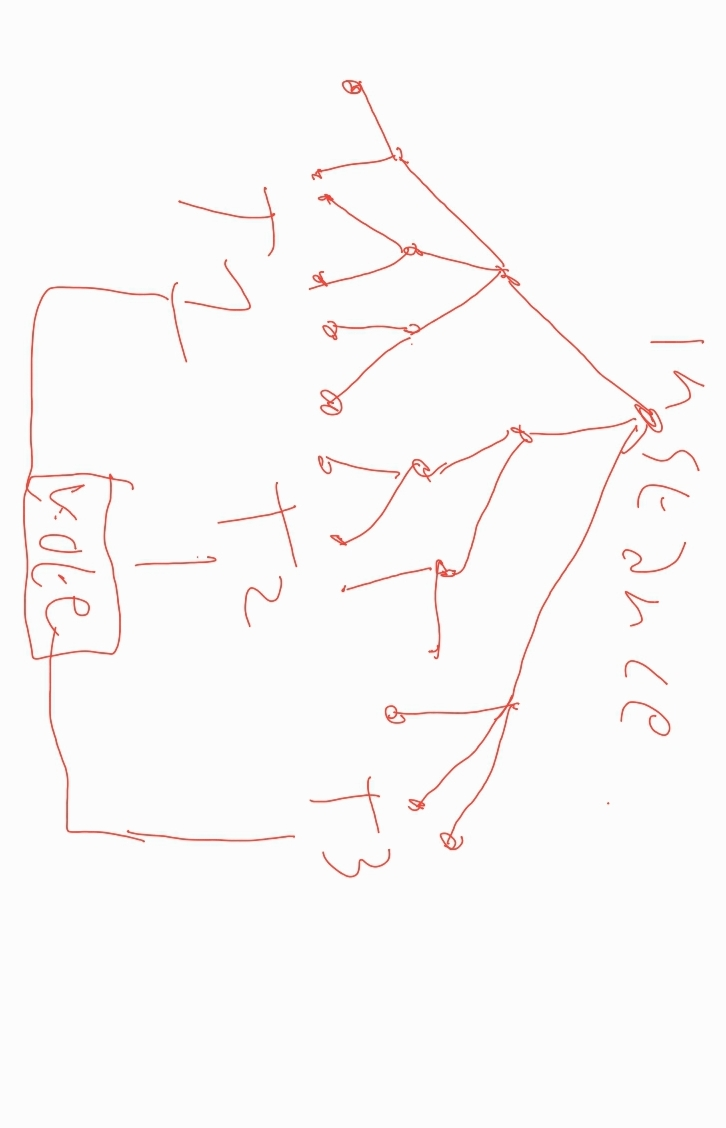
\includegraphics[scale=0.2]{figures/1174035/chapter3/random_forest.jpeg}
    \caption{Contoh Confusion Matrix}
    \label{contoh}
\end{figure}

\item Jelaskan cara membaca dataset khusus dan artikan makna setiap file dan isi field masing masing file.
Yang harus dilakukan untuk membaca dataset adalah mendownload dataset yang sudah disediakan, lalu dibuka menggunakan IDE khusus dari python seperti Spyder untuk mengetahui isi dari dataset yang sudah didownload. Tergantung dari kebutuhan, file dapat berbentuk txt ataupun csv yang sudah sering digunakan karena bentuk datanya seperti tabel dan mudah untuk digunakan. Di dalam file akan mengandung class dari field atau kumpulan data hasil penilaian yang sudah dilakukan. Total datanya sendiri bisa sampai ribuan walaupun hanyalah kategori dan status seperti 0 dan 1.


\item Jelaskan apa itu Cross Validation.
Cross Validation merupakan metode untuk mengevaluasi hasil dari sebuah penilaian yang telah digunakan dengan cara membagi dua bagian dari dataset menjadi data training dan data testing.Lalu data akan diolah sehingga muncul tingkat akurasi dari metode yang digunakan contoh pada metode random forest dataset nya di bagi menjadi dua menjadi data training dan data testing kemudian data tersebut di olah oleh mesin untuk melihat tingkat akurasinya maka akan muncul misalkan akurasi kebenaran sebesar 44 \% begitu pula dengan menggunakan metode-metode yang lain seperti decision tree dan SVM.


\item Jelaskan apa arti score 44 \% pada random forest, 27 \% pada decision tree dan 29 \% dari SVM.
Maksud dari score 44 \% tersebut yaitu nilai ketepatan atau kebenaran dari sebuah parameter, tingkat ketepatan tersebut berpengaruh pada bagaimana mesin tersebut bisa menyatakan jenis burung tersebut dengan akurasi kebenaran 44 \%. sedangkan pada metode decision tree yaitu 27 \% yang berarti menunjukan bahwa tingkat akurasi ketepatan mesin jika mengerjakan sesuatu atau menyatakan keputusan dengan metode decision tree maka nilai kebenarannya bernilai 27 \%. sedangkan dengan menggunakan metode SVM menunjukan hasil 29 \% yang berarti nilai ketepatan atau kebenaran dalam memecahkan masalah menggunakan metode SVM ini sebesar 29 \% . maka dari itu dapat di simpulkan bahwa dengan menggunakan metode random forest mesin dapat memecahkan masalah lebih akurat dibandingkan dengan menggunakan decision tree dan SVM.


\item Jelaskan bagaimana cara membaca confusion matriks dan contohnya memakai gambar atau ilustrasi sendiri.
Cara untuk membaca confusion matrix adalah dengan cara memasukan parameter nilai yang ada pada datasets. Contoh pada dataset terdapat class yang disandingkan dengan nama burung untuk di normalisasi maka akan menunjukan nilai matrix yang mendekati nilai benar dalam bentuk angka misalkan 0,5 0,2 dan seterusnya mendekati nilai satu. di karenakan susahnya membaca nilai angka maka sering di ubah menjadi bentuk grafik. Untuk nilai - nilai yang ada, adalah sebagai berikut : 
\begin{itemize}
    \item True Positive : Data positif yang terdeteksi memiliki hasil benar
    \item False Positive : Data Positif yang terdeteksi memiliki hasil salah
    \item True Negative : Data negatif yang terdeteksi memiliki hasil benar
    \item False Negative : Data negatif yang terdeteksi memiliki hasil salah
\end{itemize}
\begin{figure}[H]
    \centering
    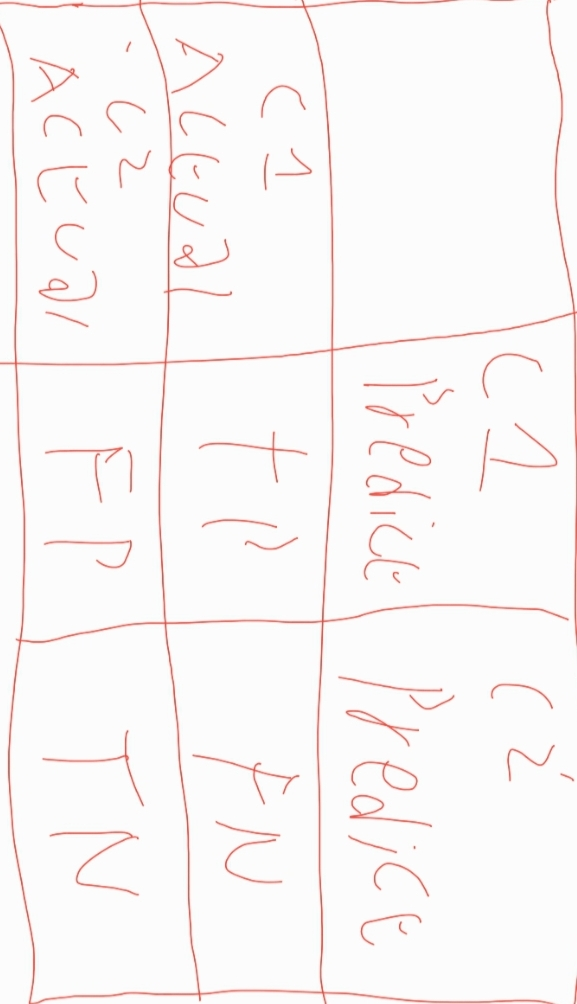
\includegraphics[scale=0.2]{figures/1174035/chapter3/confusion.jpeg}
    \caption{Contoh Confusion Matrix}
    \label{contoh}
\end{figure}


\item Jelaskan apa itu voting pada random forest disertai dengan ilustrasi gambar sendiri.\par
Voting merupakan data hasil dari decision tree yang terdapat pada random forest. Dimana hasil data tersebut di gunakan sebagai acuan untuk hasil dari random forest. sebagai contoh misalkan pada satu random forest terdapat enam decision tree untuk menentukan jenis pekerjaan orang, pada decision tree ke satu menyimpulkan bahwa pekerjaanya yaitu dosen , pada decision tree ke dua yaitu dosen kemudian pada decision tiga dosen , pada decision tree ke empat yaitu pekerja kantoran, pada decision tree ke lima yaitu pekerja kantoran dan pada decision tree ke enam yaitu dosen. maka pada random forest dapat menyimpulkan hasilnya yaitu dosen. 
\begin{figure}[H]
    \centering
    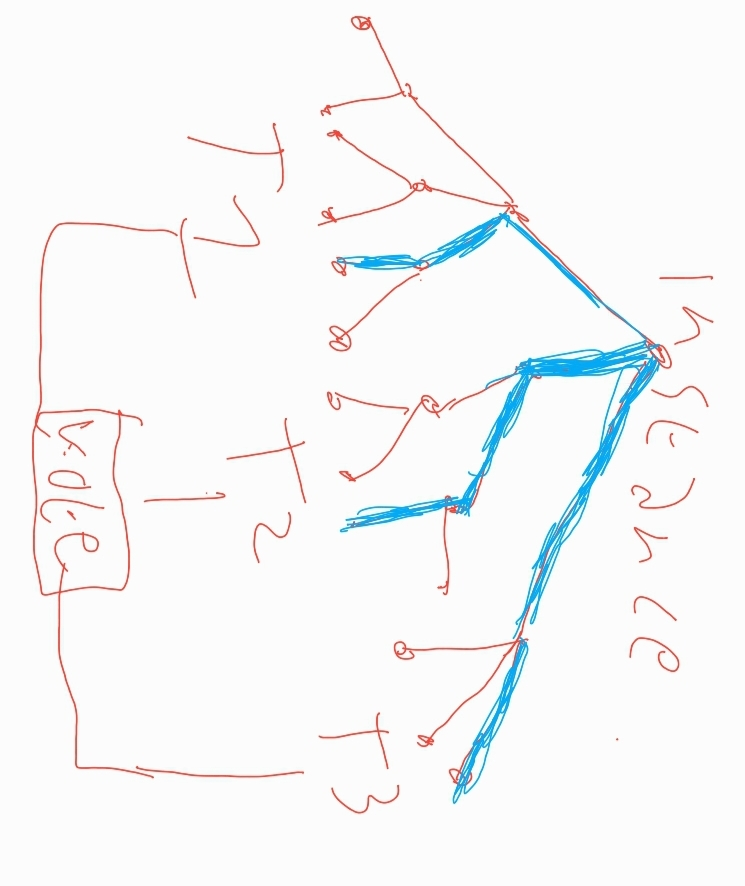
\includegraphics[scale=0.2]{figures/1174035/chapter3/random_forest_voted.jpeg}
    \caption{Contoh Random Forest yang sudah Divote}
    \label{contoh}
\end{figure}
\end{enumerate}